\chapter{架构设计}

\section{总体架构}
该系统采用的是微服务架构,即将业务拆分为多个子业务独立部署,各个子业务之间彼此独立,互相协作。同时整合网关、注册中心、负载均衡等当下流行的微服务技术,
使得各个服务之间的协作更加有合理、高效。同时为了应对集群部署,也为了提高处理速度,本系统采用Redis缓存技术,以便部分业务的处理。总体的架构图如图~\ref{fig:framework}~所示。
\begin{figure}[htbp]
    \centering
    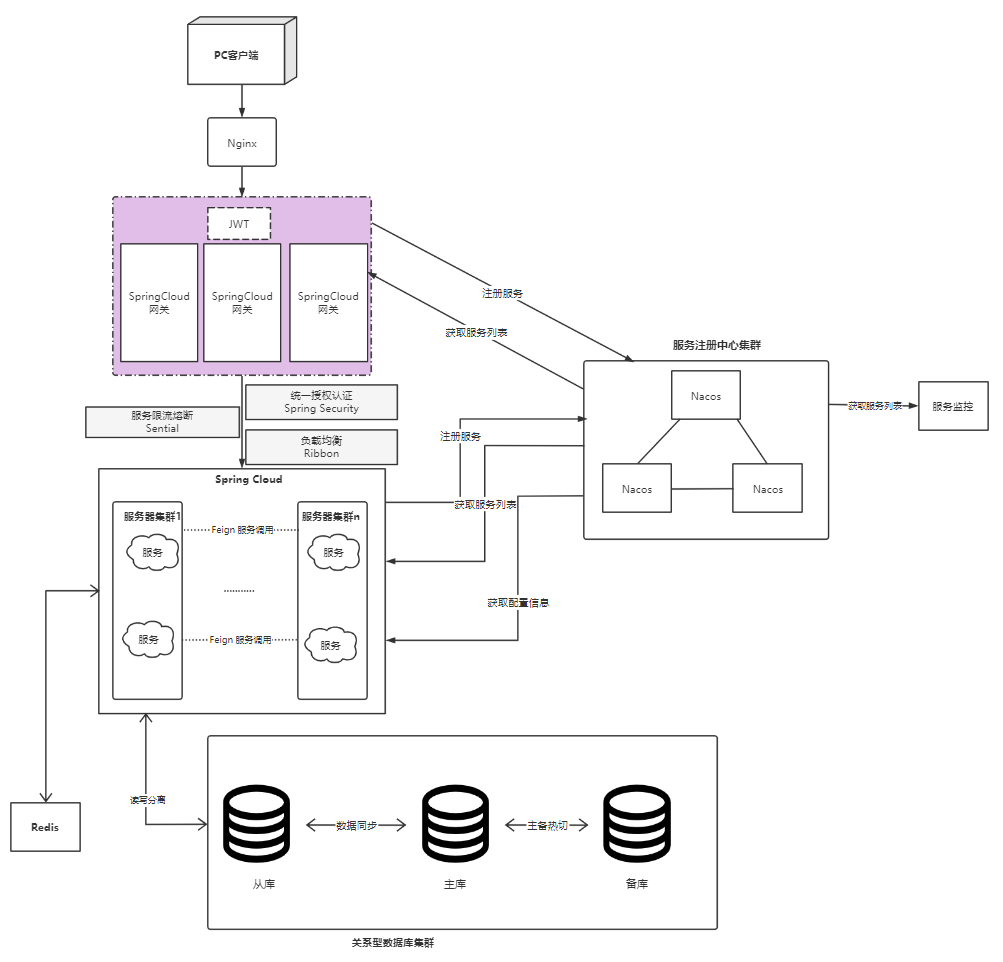
\includegraphics[width=\textwidth]{ch2/framework.png}
    \caption{总体架构}\label{fig:framework}
    \vspace{\baselineskip} % 表示图与正文空一行
\end{figure}

\subsection{具体微服务模块}
具体的微服务模块即系统给用户提供的业务服务,包括注册认证、发帖浏览等,每个具体微服务都整合了SpringCloud框架,微服务之间通过OpenFeign进行相互调用。
各个微服务集群部署,负载均衡技术采用ribbon,负载均衡策略为轮询。

\subsection{中间件}
本系统采用了许多微服务的中间件,以便更好地为微服务框架服务。
\subsubsection{服务注册与发现}
服务注册采用的是阿里巴巴开发的Nacos,部署方法为3个Nacos搭建服务注册集群。该集群可以实现各个微服务的注册,服务列表的获取和微服务的监听。
\subsubsection{服务调用}
本系统的服务调用技术采用的是OpenFeign,其为HTTP形式的REST API提供了简洁高效的RPC调用方式,同时OpenFeign也整合了负载均衡功能,便于集群之间的调用。
\subsubsection{负载均衡}
负载均衡技术使用的是Ribbon,结合OpenFeign实现微服务集群之间的互相调用,鉴于本系统的流量并不大,因此负载均衡策略采用轮询即可。
\subsubsection{网关}
网关技术使用的是Spring Gateway,他为众多服务模块提供了一个统一的访问路径,同时负责分发路由和认证授权,是所有服务调用的第一步。
\subsubsection{配置中心}
配置中心使用Nacos的配置中心,和Nacos服务注册中心紧密结合,将项目的配置文件进行统一的管理,同时也将项目的开发环境进行有效的隔离。
\subsubsection{服务降级和服务熔断}
本系统采用Sentinel技术实现服务降级和服务熔断,在流量超出服务器上限,或是出错率超过阈值时,会返回特定页面,以给客户更好的服务体验。
\subsubsection{消息队列}
本系统采用RabbitMQ实现消息队列,实现应用之间的异步调用,使得一些不需要及时反馈的操作可以异步进行,从而加快响应速度,提高用户体验。


\subsection{存储与缓存}
\subsubsection{数据库}
系统采用的为MySQL数据库,其数据模型的具体请详见后面的详细设计,会将每张数据表的字段和约束具体描述。
\subsubsection{缓存}
系统采用的是Redis缓存,其是基于内存的非关系型数据库,用于为本系统提升查询速度,主要在认证授权模块等高频模块使用。


